
\begin{figure}
\centering
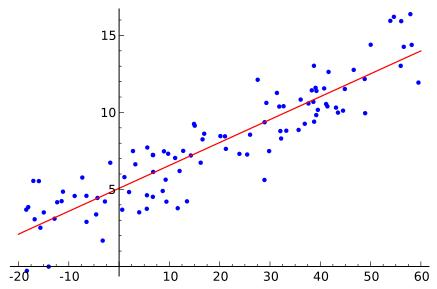
\includegraphics[width=10cm]{images/linear_regression.jpg}
\caption{Ejemplo de Regresión Lineal}
\end{figure}

\section{Análisis de regresión}

Llegado a este punto, dada una variable a/p, nos interesaría evaluar la relación entre el entrainment y las distintas variables sociales. Con esto en mente, planteamos un modelo de regresión lineal donde nuestra variable explicativa será la mimetización, y la variable \emph{dependiente} será la variable social.

En base a ésto, podremos observar cuál es la variación conjunta de ellas. Es esperable que, al aumentar la mimetización, aumenten ciertas variables sociales (por ejemplo, la compenetración en el juego) y que otras desciendan (el aburrimiento).


\subsection{Modelo clásico de Regresión Lineal}

En el modelo clásico de regresión lineal, tenemos un conjunto de valores fijos $X_1, X_2, \ldots, X_n$, que son llamadas variables independientes. Asociado a cada uno de estos valores fijos, tenemos variables aleatorias $Y_1, \ldots, Y_n$. Asumimos, además, que nuestras variables son de la forma

\begin{equation}
  Y_i = E[Y|X_i] + u_i
\end{equation}

donde $u_i$ es la perturbación estocástica de la variable.

Asumiendo que $E[Y|X_i]$ es una función lineal de $X_i$; es decir, que existen $\beta_1, \beta_2 \in \mathbb{R}$ que cumplen

\begin{equation}
  E[Y|X_i] = \beta_1 + \beta_2 X_i
\end{equation}

obtenemos que

\begin{equation}
  Y_i = \beta_1 + \beta_2 X_i + u_i
\end{equation}

Nuestro objetivo es poder entonces conseguir estimadores $\widehat{\beta_1}, \widehat{\beta_2}$ que nos permitan analizar y predecir el comportamiento conjunto de estas variables.

\subsection{Nuestro modelo}

Sea entonces una variable acústica/prosódica (por ejemplo, el pitch o la intensidad), y una variable social de las que acabamos de enumerar en \ref{sec:panel_data}. Sean $E_1, \ldots, E_n$ los valores de entrainment para el set de datos que definimos en \ref{sec:panel_data}, y sean $V_1, V_2, \ldots V_n$ los valores de la variable social de cada conversación.

Sobre éstas variables es que planteamos nuestro modelo de regresión lineal clásica: queremos ver qué relación hay tomando como variable ``fija'' al entrainment, y como variable dependiente a la variable social. Queremos hallar, entonces $\widehat{\beta_1}, \widehat{\beta_2} \in \mathbb{R}$

\begin{equation}
  V_i \simeq \widehat{\beta_1} + \widehat{\beta_2} E_i
\end{equation}


Para ello, calcularemos los estimadores $\widehat{\beta_1}, \widehat{\beta_2} \in \mathbb{R}$ mediante el método \emph{QR} (insertar referencia aquí) que nos provee el lenguaje R. A su vez, luego de ésto efectuaremos un análisis de significancia sobre $\beta_2$ para verificar que sean distintos de 0.


Uno esperaría que un alto \emph{entrainment} se relacione con un alto valor de ciertas variables sociales \cite{BRE1996}, por ejemplo la compenetración con el juego, el ayudar a terminarlo. Esto significa esperar que el valor de $\widehat{\beta_2}$; y se relacione con bajos valores de otras, como el aburrimiento, o el rechazo percibido hacia el compañero.


\subsection{Modelo agrupado o \emph{pooled}}

En el modelo agrupado o \emph{pooled}, no distinguimos entre datos provenientes de distintos ``grupos'' \cite{gujarati1999} y sobre éstos calculamos la regresión lineal, agrupando todos los datos disponibles.

Un problema que surge con este tipo de regresión es que niega todo tipo de \emph{heterogeneidad} de los datos: estos pueden provenir de interlocutores más o menos empáticos, o cuya interacción en el juego se vio influída por factores no medidos en el experimento. Todo ésto es descartado, aún cuando puede afectar seriamente  el resultado obtenido.

AGREGAR GRAFICO DE EJEMPLO PARA ESTO

\subsection{Modelo de Efectos Fijos dentro de cada grupo}


El modelo de efectos fijos agrega el concepto de heterogeneidad permitiendo que cada sujeto tenga su propio valor de ordenada al origen. En términos formales, reformulemos nuestro modelo de la sección anterior:

\begin{equation}
  V_{it} = \beta_1 + \beta_2 * E_{it} + u_{it}
\end{equation}

donde $i$ es la cantidad de sujetos (en nuestro caso, 12 sesiones por 2 interlocutores = 24), $t$ es la variable de tiempo (en nuestro caso, las tareas de cada sesión). El modelo de efectos fijos nos permite


DEFINIR SUJETO

